\documentclass[12pt]{article}
\usepackage[a4paper,top=2cm,bottom=2.2cm,left=3cm,right=3cm,marginparwidth=1.75cm]{geometry}
\usepackage{amsmath,amsthm,amssymb}
\usepackage[spanish]{babel}
\usepackage{listings}
\usepackage{csvsimple,booktabs}
\usepackage{filecontents}
\usepackage{amsmath}
\usepackage{graphicx} % figuras
\usepackage{subfigure} % subfiguras
\usepackage{color}
\usepackage{cite}
\definecolor{mygreen}{rgb}{0,0.6,0}
\definecolor{mygray}{rgb}{0.5,0.5,0.5}
\definecolor{mymauve}{rgb}{0.58,0,0.82}
\usepackage[colorinlistoftodos]{todonotes}
\usepackage[colorlinks=true, allcolors=blue]{hyperref}
\usepackage{movie15}
\usepackage[utf8]{inputenc}
\lstdefinestyle{tt}{language=Python, literate= {á}{{\'a}}1 {ó}{{\'o}}1 {ñ}{{\~n}}1, breaklines=true, basicstyle={\small}, commentstyle=\color{red}, frame=single, extendedchars=true, otherkeywords={True, False}, keywordstyle=\color{mymauve}, columns=flexible, stringstyle=\color{mygreen}, breakatwhitespace=true, numbers=left, numberstyle=\scriptsize\color{mygray}, tabsize=3, rulecolor=\color{black}}
\lstdefinestyle{rm}{language=R, commentstyle=\color{mygray}, keywordstyle=\color{blue}, stringstyle=\color{mygreen}, breakatwhitespace=true, breaklines=true, columns=flexible, extendedchars=true, literate={ó}{{\'o}}1 {ú}{{\'u}}1 {ñ}{{\~n}}1 }
\begin{document}
\title{{\LARGE \textbf{Experimentos con el algoritmo de Floyd-Warshall en \texttt{python}}}\\ {\large Yessica Reyna Fernández}\\{\large Flujo en Redes}}
\maketitle
\section{Introducción}
En un grafo se pueden denotar la forma de relacionarse con otras personas, entonces si se formara un circulo con un determinado número de personas, todos pueden ver a todos, pero no cualquiera puede hablar o conversar con todos los que están en la circunferencia que se ha formado, ya que por la lejanía se genera ruido y no se puede transmitir de buena manera algún mensaje determinado, es por eso que de cierta manera solo se podría interactuar primeramente con el más próximo que es las dos personas a los lados y algunas más que son sucesivas a las próximas, dicho esto es una forma de interpretación a la nueva modelación de grafo que se genera y da explicación en las siguientes secciones y la forma de ver estas relaciones o conexiones en formas de aristas que perciben una distancia entre cada par de personas o nodos y que otras características más podrían ser validad para alguna relación que pueda ser interpretada por el grafo en particular.\\Todo siguiendo la estructura para la realización de grafos prevista por la practica 3\cite{mio}.
\section{Grafo circular base}
Primeramente con respecto a la posición de los nodos, se posicionan en forma de circunferencia, entonces se realiza la transformación a coordenadas en radianes para la circunferencia a formar; a continuación se debe definir en ese caso la posición del ángulo en donde ira cada punto para esta transformación por lo cual se deberá tomar una medida equitativa para la cantidad de nodos que se tiene, tomando en cuenta la ecuación paramétrica de la circunferencia con centro en $(a,b)$ donde $x=a+rCos(t)$ y $y=b+rSen(t)$ con $t\in[0,2\pi]$, definiendo lo siguiente como parte básica del grafo:
\begin{lstlisting}[style=tt]
angulo=2*pi/n #n=cantidad de nodos
r=0.3 #radio fijo de la circunferencia
c=(0.5,0.5) #posición del centro de la circunferencia
self.pos[v] = (c[0]+(r * cos(angulo * v)), c[1]+(r* sin(angulo * v))) #dentro de la función nodoscrear() con v=indice del nodo a crear
\end{lstlisting}
Ahora bien hablando de la forma de trazar las aristas entre nodos se mide en forma de un parámetro $k$, el cual varía dependiendo de la cantidad de nodos; por lo que se busca que cada vez que se corra el código las repeticiones que habrá de cada tamaño este dada por el valor $ \lfloor n/2 \rfloor $ ademas de que el valor de $k$ realiza las conexiones entre nodos; asimismo se define \texttt{E[(u,v)]} como las distancias euclidianas entre cada par de nodos y \texttt{vecinos[v].add(i+(j+1))} lo que agrega al nodo $i+(j+1)$  entre los vecinos de $v$, todo esto descrito en lo siguiente:
\begin{lstlisting}[style=tt]
def conecta(self, k) #función de conexiones en aristas
	for j in range(k): #recorrer tamaño de k
		for i in range(len(self.V)): #recorriendo cada nodo
			if i< (len(self.V)-(j+1)): #siempre que el indice no pase el valor k
				self.E[(i, i+(j+1))] = self.E[(i+(j+1), i)]=self.euclidiana(i,(i+(j+1)))
				self.vecinos[i].add(i+(j+1))
				self.vecinos[i+(j+1)].add(i)
\end{lstlisting}
En relación con esto se define la función para integrar aristas aleatorias al grafo que depende de una probabilidad que aumenta con el valor de $k$, agregando esa nueva arista siempre que no se encuentre considerada en él, además de que su probabilidad para entrar al grafo sea más pequeña que un número que se genera aleatoriamente:
\begin{lstlisting}[style=tt]
prob=2**-(k)
def conectaaleatorio(self, prob)
	if m is not w and (m,w) not in self.E:
		if random()< prob:
			self.E[(m,w)]=self.E[(w,m)]=self.euclidiana(m,w)
			self.vecinos[m].add(w)
			self.vecinos[w].add(m)
\end{lstlisting}
Así pues, esto definiría lo más básico por elaborar par aun grafo base circular, tratando en las siguientes secciones otros aspectos que se pueden agregar al grafo.
\section{Promedios de distancias}
Como se ha tratado en prácticas anteriores, el algoritmo de Floyd-Warshall\cite{libroalgo} crea un vector con todos los pares de distancias entre un par de puntos dados $u$ y $v$.\\
Por lo cual se puede considerar como característica en el grafo lo que sería el promedio de distancias entre nodos, tomando la suma de distancias de todos los pares de nodos dados obteniendo así este parámetro que varía dependiendo de la cantidad de nodos, esto es, $D= \frac{\sum_{i=1}^n d[i]}{n}$, donde \texttt{d[i]} es el vector de las distancias tomado del algoritmo de Floyd-Warshall.\\ Donde todo lo ya dicho se desglosa en las siguiente líneas de código:
\begin{lstlisting}[style=tt]
def promediodistancias(self):
	self.suma = 0
	for key, value in self.d.items():
		self.suma= self.suma+value
	return self.suma/n
\end{lstlisting}
Acto seguido a esto se define una nueva función matemática, la cual en relación con los valores de $n$ y de $k$, se crea una cota superior al valor de la distancia promedio que se calculó con anterioridad.\\
Hablando un poco más de ella, esta se calcula en base a la longitud del vector de distancias, el cual crece conforme al valor de $n$, entre el cociente de la mitad de las interacciones que hay de nodos y la longitud de la circunferencia.\\Dicho de otra manera, se mostrara a continuación las líneas de código pertenecientes a la descripción de la formulación de la cota superior para la normalización de las distancia promedio del grafo conforme a la cantidad de nodos y el valor de interacción entre ellos $k$, asimismo nos indica si para algún valor de $n$ y de $k$ no se llega a cumplir el valor de la cota y se pueda realizar el ajuste de esta:
\begin{lstlisting}[style=tt]
def cota(self):
	circumferencelength= 2*(pi)*r
	supremo=(((n**2)-n)/((0.5)*k))*circumferencelength
	if supremo> self.suma/n:
		return (self.suma/n)/supremo
	else:
		print(n, k)
		print("No es buena cota")
\end{lstlisting}
\section{Densidad de cluster}
Como otro rasgo a denotar para un grafo se puede considerar la densidad de cada uno de sus cluster o grupo su equivalente en español, el cual indica el número de conexiones que debería existir por grupo que forma cada uno de los nodos individualmente, es decir, quienes de sus vecinos está conectado entre ellos mismos.\\
Formulando esto matemáticamente se obtendría un coeficiente de densidad de grupo en un rango de $(0,1)$ con la siguiente formula: $C=\frac{2m}{n(n-1)!}$.\\ Obteniendo esto en el código con las siguiente líneas, en donde al formar una doble iteración en la lista de los vecinos de $v$ se evita poner el dos de la formula y dividiendo al final entre la cantidad de nodos generados:
\begin{lstlisting}[style=tt]
def promclusters(self):
	csuma=0
	for v in range(len(self.V)):
		m=0
		for i in self.vecinos[v]:
			for b in self.vecinos[v]:
				if b in self.vecinos[v]:
					m += 1
					csuma += m/(n*(n-1))
	return csuma/len(self.V)
\end{lstlisting}\pagebreak
\section{Resultados}
El objetivo principal de la practica era verificar el comportamiento del tiempo que se toma el algoritmo implementado en resolverse y comprobar así que se sigue manteniendo el mismo comportamiento de tiempo computacional empleado por el algoritmo de Floyd-Warshall, asimismo como interpretar los datos obtenidos por las nuevas características del grafo agregadas para uso de esta práctica y así demostrar algún tipo de comportamiento que se relacione entre la cantidad de nodos a considerar y las variaciones de conexiones entre pares de nodos.\\
Entre las siguientes figuras se mostrara la relación de los tiempos tomados para los diferentes cantidades de nodos que se verá en la figura \ref{Figura 1:}, hay que destacar que al analizar la gráfica generada por los tiempos esta sigue manteniendo el mismo tiempo computacional referido del algoritmo mismo de $\mathcal{O}$$(n^3)$.
\\Acto seguido se apreciaran los gráficos generados para las distancias promedio y las densidades de cluster realizados para cada cantidad de nodos graficadas contra la probabilidad con la que se varió las conexiones intermedias de nodos en una escala logarítmica en un intervalo de $(0,\frac{1}{2^1})$ en la figura \ref{Figura 2:} y la figura \ref{Figura 3:}.\\
\begin{figure}[h!]
	\centering
	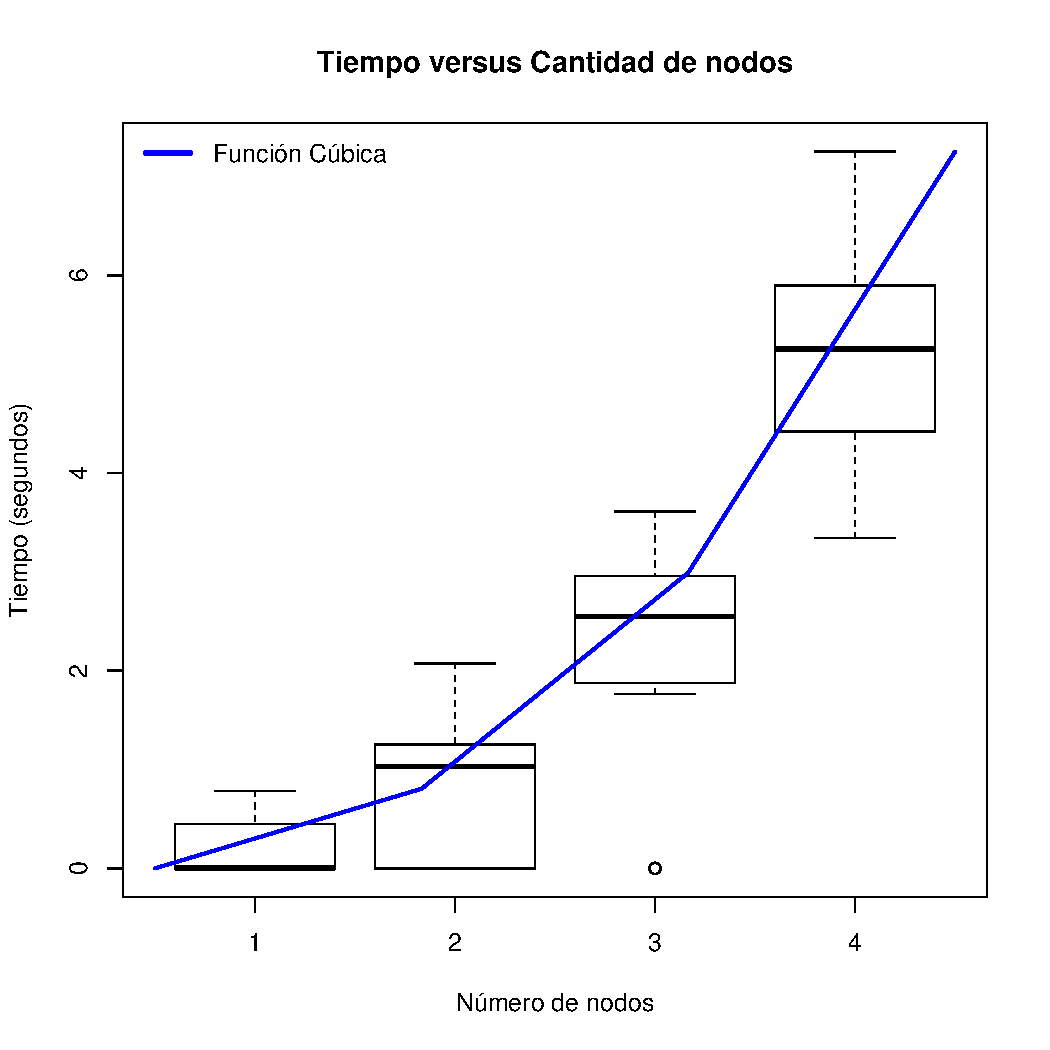
\includegraphics[width=0.6\textwidth]{TiempovsN}
	\caption{Tiempo versus Cantidad de nodos\label{Figura 1:}}
\end{figure}\pagebreak
\\Para la gráfica anterior se hace uso del lenguaje de programación \texttt{R}\cite{R} con apoyo de los archivos tipo \texttt{csv} con los datos de los tiempos para cada cantidad diferente de nodos, verificando la normalidad de los datos y ajustando la curva de esfuerzo computacional del algoritmo a los datos analizados en un diagrama de cajas, todo esto se resume con las siguientes líneas de código:
\begin{lstlisting}[style=rm]
Tiempos <- as.data.frame(t(read.csv("Tiempo60.csv", header=FALSE)))
T90<-as.data.frame(t(read.csv("Tiempo90.csv", header=FALSE)))
T120<-as.data.frame(t(read.csv("Tiempo1.csv", header=FALSE)))
T150<-as.data.frame(t(read.csv("Tiempo150.csv", header=FALSE)))
TTotales<-t(smartbind(Tiempos, T90, T120, T150,fill=0))
shapiro.test(TTotales)#no normales
pdf("TiempovsN.pdf")
boxplot(TTotales, main="Tiempo versus Cantidad de nodos", xlab=c("Número de nodos"), ylab=c("Tiempo (segundos)"), varwidht=TRUE, notch=FALSE, plot=TRUE)
par(new=TRUE, pty="m", xaxt="n", yaxt="n")
plot(seq(1:4)^3, type="l" , xlab="", ylab="", col="blue", lwd=2)
legend("topleft",col=c("Blue"), legend =c("Función Cúbica"), lwd=3, bty = "n")
graphics.off()
\end{lstlisting}\pagebreak
Mientras tanto que las siguientes gráficas fueron realizadas en \texttt{gnuplot} apartir del archivo dentro del repositorio llamado \texttt{grafica.py}\cite{grafica}
\begin{figure}[h!]
	\centering
	\subfigure[$n=60$.]{\includegraphics[width=0.70\textwidth]{imgen60}}
	\subfigure[$n=90$.]{\includegraphics[width=0.70\textwidth]{imgen90}}
	\caption{Distancia promedio/cota y densidad de cluster.}\label{Figura 2:}
\end{figure}
\pagebreak
\begin{figure}[h]
	\centering
	\subfigure[$n=120$.]{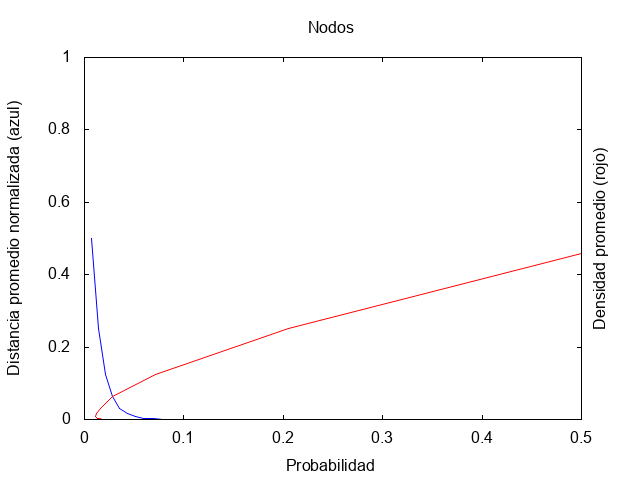
\includegraphics[width=0.70\textwidth]{imgen}}
	\subfigure[$n=150$.]{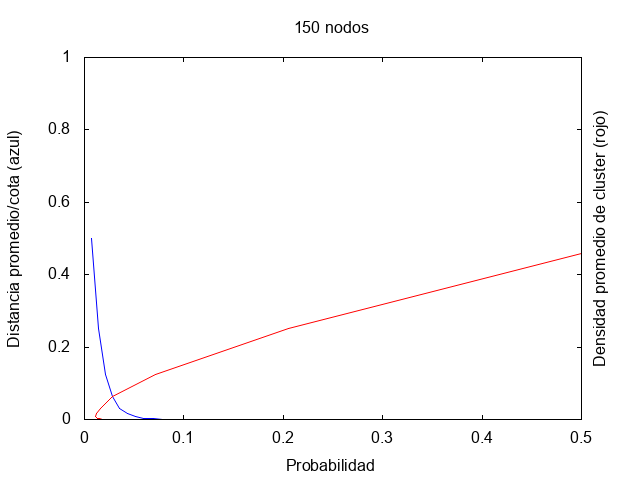
\includegraphics[width=0.70\textwidth]{imagen150}}
	\caption{Distancia promedio/cota y densidad de cluster.}\label{Figura 3:}
\end{figure}\pagebreak
\\En conclusión se puede asegurar que con forme la cantidad probabilidad de conexiones aumenta, es decir, hay más aristas en el grafo respecto a la distancia promedio generada por todos los pares de distancias toma valores cada vez más pequeños ya que la distancia decrece a grandes rasgos ya que hay más diferentes tipos de aristas por considerar, para la creación de distancias entre pares de nodos, lo cual las acerca más unos entre otros.\\En lo cual el caso de la densidad de cluster o agrupación es un caso contrario, ya que entre más conexiones haya por nodo, habrá más posibilidad de que los vecinos del mismo tengan aristas entre ellos o la diferencia entre la cantidad de aristas que deba haber entre ellas a las que en realidad exista sea cada vez más pequeña.
\bibliographystyle{unsrt}
\bibliography{mibliblio}
\end{document}
